%--------------------------------------------------------------------------------------------------
% 
\chapter{Data Description}
\label{ch:data}
%--------------------------------------------------------------------------------------------------
Write introduction

\section{Data Preparation}

The dataset we used in our experiments comprises news articles labelled by the news monitoring industry, which tracks news outlets across six Central European and Western Balkan countries.

\begin{table}[h!]
\centering
\caption{List of Selected Industries}
\label{tab:industries}
\centering
    \resizebox{0.4\textwidth}{!}{%
        \begin{tabular}{l}
            Manufacturing \\
            Information and Communication Technology \\
            Healthcare and Pharmaceutical\\
            Finance and Insurance\\
            Foods and Agriculture\\
            Energy\\
            Retail\\
            Transportation\\
            Media and Entertainment\\
            Politics and Religion\\
            Automotive\\
		\end{tabular}
}
\end{table}

To obtain as diverse a representation of news media language as possible, we sampled the articles from January 2023 until December 2023, using labels corresponding to different industries monitoring news (see Table~\ref{tab:industries}). 
This sampled $NewsMon$ dataset comprises one million articles from eight countries (Serbia, Slovenia, Bosnia and Herzegovina, Croatia, Macedonia, Montenegro, Kosovo, and Albania) in more than seven languages (see Figure~\ref{fig:languages_hist}).
It is annotated with more than twelve thousand distinct labels. 
It encompasses all labels, not just the "seed" labels from the selected industries used for the initial selection.

\begin{figure}[h!]
  \centering
  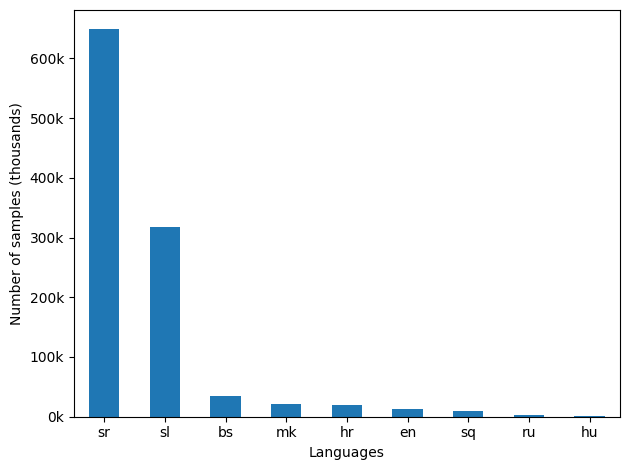
\includegraphics[width=0.5\textwidth]{figures/languages_hist.png}
  \caption{The distribution of languages across all samples (Serbian, Slovene, Bosnian, Macedonian, Croatian, English, Albanian, Russian and Hungarian).}
  \label{fig:languages_hist}
\end{figure}

Each article is assigned labels representing concepts or topics of interest to end-users.
Despite the system's vast number of labels, each end-user typically monitors only a few.
Each label is associated with several simplified Keyword-Boolean Expressions (KwEs) that determine the initial assignment of labels to news articles. 
News articles are automatically labelled based on those KwEs in the intake processing pipeline. 
At the final stage of the intake processing pipeline, a human moderator reviews the labels assigned to each article, as illustrated in Figure~\ref{fig:monitoring_flow}.
The moderator may confirm, reject, or add additional labels based on their assessment.
Labels and their corresponding KwEs are updated whenever a new user joins or leaves or when end-user interests change.
These updates can occur frequently, averaging about one hundred monthly label changes.
Arbitrary labels are also added at later stages by the analysis department.

\begin{figure}[h!]
  \centering
  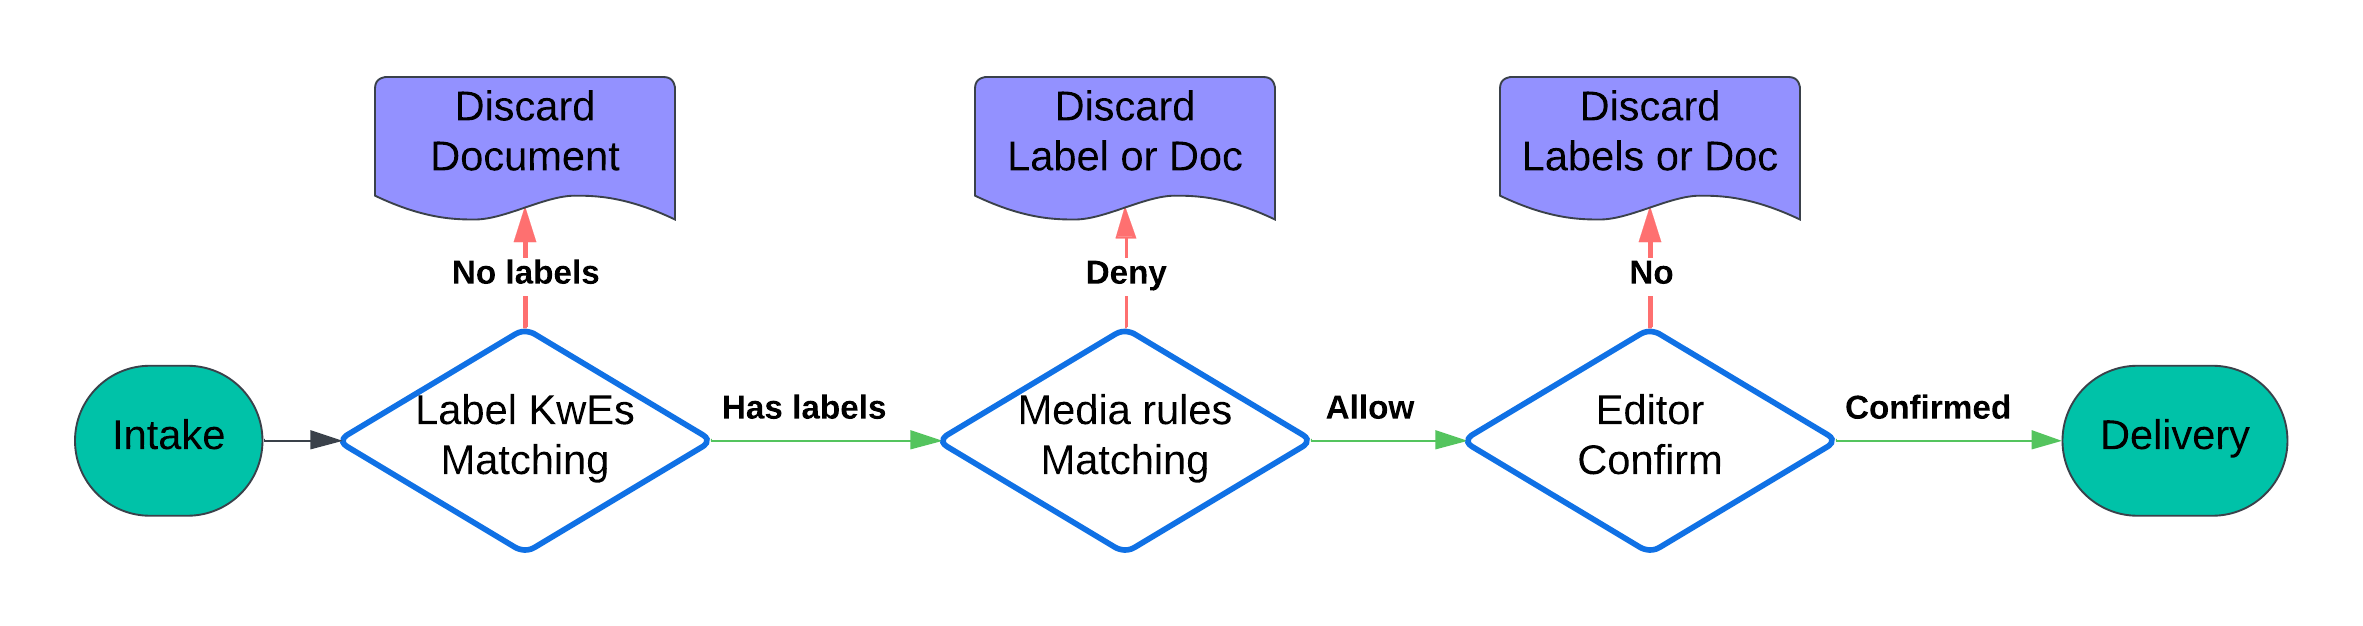
\includegraphics[width=0.9\textwidth]{figures/monitoring_flow.png}
  \caption{News monitoring intake processing pipeline.}
  \label{fig:monitoring_flow}
\end{figure}

\renewcommand{\arraystretch}{1.5}
\begin{table}[htb]
    \caption{Examples of simplified Keyword-Boolean Expressions}
	\label{tab:frames}
	\centering
    \resizebox{\textwidth}{!}{%
		\begin{tabular}{l|l}
            \hline
            \textbf{Keyword Expression}& \textbf{Explanation}\\
            \hline
            \hline
            \textbf{tesla OR teslo OR tesli OR tesle -"nikol* tesl*"}& Match the Tesla car brand if Nikola Tesla the person is not present in text\\
            \hline
            \textbf{mercedes* -formul* -"max verstap*" -F1 ...}& Match the Mercedes car brand if Formula 1 terms are absent.\\
            \hline
            \textbf{nlb* -"lig* nlb" -"nlb lig*"}& Match all forms of NLB terms, but only if NLB-sponsored league is not present.\\
            \hline
            \textbf{gradnj* -cest* -avtocest* -obvoznic*}& Match the term construction without the terms: road, highway or ring road\\
            \hline
            \textbf{\foreignlanguage{russian}{"сенад* софтић*"} OR "senad* softić*"}& Match the person with various inflections and in various scripts\\
            \hline
		\end{tabular}
  }
\end{table}
In the second iteration of data gathering, we collected the KwEs from moderator-confirmed labels along with their re-matched text spans.
Re-matched text spans provide an opportunity to pinpoint relevant text for specific labels, which could help address the issue of text truncation in specific targeted Transformer models and give us an opportunity for an effective information retrieval approach. 
Unfortunately, some labels still exist without their KwEs directly occurring in the text.
Upon further examination, we observed that the labels fall into two broad classes:
\begin{itemize}
  \item \textbf{Named Entities (NE)}: mostly Persons, Organizations, Products, Brands and rarely Locations.
  \item \textbf{General Concepts (GC)}: a set of terms representing a concept, for example, E-Mobility, Health insurance, Climate Change, Industrial waste.
\end{itemize}
We also found numerous labels with KwEs, most often from the NE class, that would match the same text.
These duplicates could potentially be removed, or the classification process optimized for the NE class of labels.
Some labels, especially from the GC class, are often context-dependent. 
For example, while the "Competition" label applies to many industries and seems like a duplicate, its meaning and KwEs vary depending on the context.
We further removed titles from the news article body text where present and combined them with the title to obtain a complete text.

\section{Data Analysis}

Due to the large dataset and label set size, we decided to down-sample the $NewsMon$ data, obtaining the $NewsMon_{sl}$ to speed up our research cycle for testing different classification methods and techniques.
We focused on publicly available Slovene data from January 2023 to May 2023, aiming for a dataset size and label distribution similar to other well-known multi-label datasets.
Next, we removed the labels that appear only once to prepare the $NewsMon_{sl+cls}$ dataset for baseline classifier training.
Below are some of the most popular datasets used for multi-label text classification we considered for comparison~\parencite{li2022surveytextclassification, tarekegn2024deeplearningmultilabellearning}:
\begin{itemize}
\item \textbf{Reuters-21578}: 
This widely-used dataset is derived from Reuters financial news services. 
It includes 90 classes containing 7,769 training texts and 3,019 testing texts (ApteMod corpus) containing single and multiple labels. 
Variants include subsets like R8 and BR52~\parencite{lewis1997reuters}.
\item \textbf{RCV1}, \textbf{RCV1-v2}, and \textbf{RCV1-2K}:
The Reuters Corpus Volume I (RCV1) comprises articles from Reuters News in 23 languages, collected between 1996 and 1997. 
It has 103 categories, featuring 23,149 training texts and 784,446 testing texts. RCV1-v2 includes corrections to the original dataset, while RCV1-2K expands the label set to 2,456 labels~\parencite{lewis2004rcv1}. With neural network approaches, test and train sets are usually swapped.
\item \textbf{AAPD (Arxiv Academic Paper Dataset)}: AAPD contains 55,840 academic papers from the Arxiv website, with abstracts and corresponding subjects labelled with 54 categories~\parencite{clement2019arxiv}.
\item \textbf{EURLEX57K}: EURLEX57K consists of 57,000 legislative documents from EUR-LEX. 
Each document is organized into four sections: the header (title and legal body), recitals (legal background), main body (usually articles), and attachments (e.g., appendices, annexes). 
The documents are annotated with concepts from EUROVOC, which includes around 7,000 labels. However, only 4,271 (59.31\%) of these are present in EURLEX57K, and just 2,049 (47.97\%) have been assigned to more than 10 documents.~\parencite{chalkidis-etal-2019-large}.
\item \textbf{AmazonCat-13K}: AmazonCat-13K is a large-scale multi-label text classification dataset commonly used for benchmarking extreme multi-label classification algorithms. The dataset consists of product titles and descriptions from Amazon. It contains 1,186,239 training samples and 306,782 test samples with 13,330 possible labels/categories. The average number of labels per sample is 5.04~\parencite{mcauley2013hidden}.
\end{itemize}

We specifically chose to compare our dataset with the $EURLEX57K$ dataset, a large-scale multi-label text classification (LMTC) dataset with properties similar to our down-sampled version regarding the label and instance size.
More importantly, comparing our dataset to the $EURLEX57K$ dataset allows us to evaluate the performance of our baseline classifiers in Chapter~\ref{ch:retrieval}.
We used $EURLEX57K$ model evaluation metrics to assess how well the same baseline model performs when trained on our dataset, considering our datasets consist of a lesser-used language in the model pretraining.
To do so, we first introduce label distribution metrics and then analyze the similarities and differences between the two datasets.

\subsection{Label Distribution Metrics}
To compare the datasets, we employed common label distribution metrics~\parencite{TAREKEGN2021107965, Bernardini2014CardinalityAD}.
We define Label Cardinality as the average number of labels per sample:
\begin{equation}
\text{Card}(M) = \frac{1}{m} \sum_{i=1}^{m} |Y_i|
\end{equation}
Label Density as the average number of labels per instance divided by the total number of  labels:
\begin{equation}
\text{Dens}(M) = \frac{1}{m} \sum_{i=1}^{m} \frac{|Y_i|}{|L|}
\end{equation}
and finally, Label Diversity as a number of distinct label combinations in the sample set:
\begin{equation}
\text{Diver}(M) = |{Y_x \subseteq L: (x, Y_x) \in M}|
\end{equation}
Where $M$ is the multi-label dataset, $m$ is the number of instances in $M$ (i.e., $m = |M|$), $Y_i$ is the set of labels for the $i$-th instance, and $L$ is the set of all possible labels in the dataset.

\subsection{Comparison}

All three datasets $NewsMon_{sl}$, $NewsMon_{sl+cls}$, and $EURLEX57K$ exhibit a long-tail label distribution, where most labels occur infrequently. 
They contain a large number of instances (ranging from 57,000 to 62,049) and a diverse set of labels (from 3,339 to 4,271).

\begin{table}[h]
    \centering
    \begin{tabular}{lrrrrr}
        \hline
        \textbf{Dataset} & \textbf{Samples} & \textbf{Labels} & \textbf{Cardinality} & \textbf{Density} & \textbf{Diversity} \\
        \hline
        \hline
        $NewsMon$ & 1,068,261 & 12,305 & 3.392 ± 4.017 & 0.00028 & 267,564 \\
        $NewsMon_{seed}$ & 1,068,261 & 1,960 & 2.213 ± 2.316 & 0.00114 & 183,361 \\
        $NewsMon_{sl}$ & 62,049 & 4,052 & 3.034 ± 3.492 & 0.00075 & 17,307 \\
        $NewsMon_{sl+cls}$& 62,049 & 3,339 & 3.023 ± 3.470 & 0.00091 & 17,202 \\
        \hline
        $EURLEX57K$ & 57,000 & 4,271 & 5.069 ± 1.701 & 0.00119 & 34,982 \\
        \hline
    \end{tabular}
    \caption{Shows the dataset statistics for the complete set ($NewsMon$), selected seed-set of labels ($NewsMon_{seed}$), the down-sampled dataset in Slovene ($NewsMon_{sl}$), and the down-sampled dataset with single occurrence labels removed ($NewsMon_{sl+cls}$).}
    \label{tab:dataset_statistics}
\end{table}

The $NewsMon_{sl}$ dataset includes 62,049 instances and 4,052 labels, with an average of 3.034 labels per instance. 
The label density is 0.00075, indicating that labels are distributed sparsely across the dataset.
The derived $NewsMon_{sl+cls}$ dataset also consists of 62,049 instances but with 3,339 labels, as single-occurrence labels were removed during filtering. 
Since we removed single occurring labels, the result is unsurprisingly a slightly lower average of 3.023 labels per instance but a higher label density of 0.00091, reflecting a more concentrated label distribution after filtering (see Table~\ref{tab:dataset_statistics}).

\begin{figure}[h!]
  \centering
  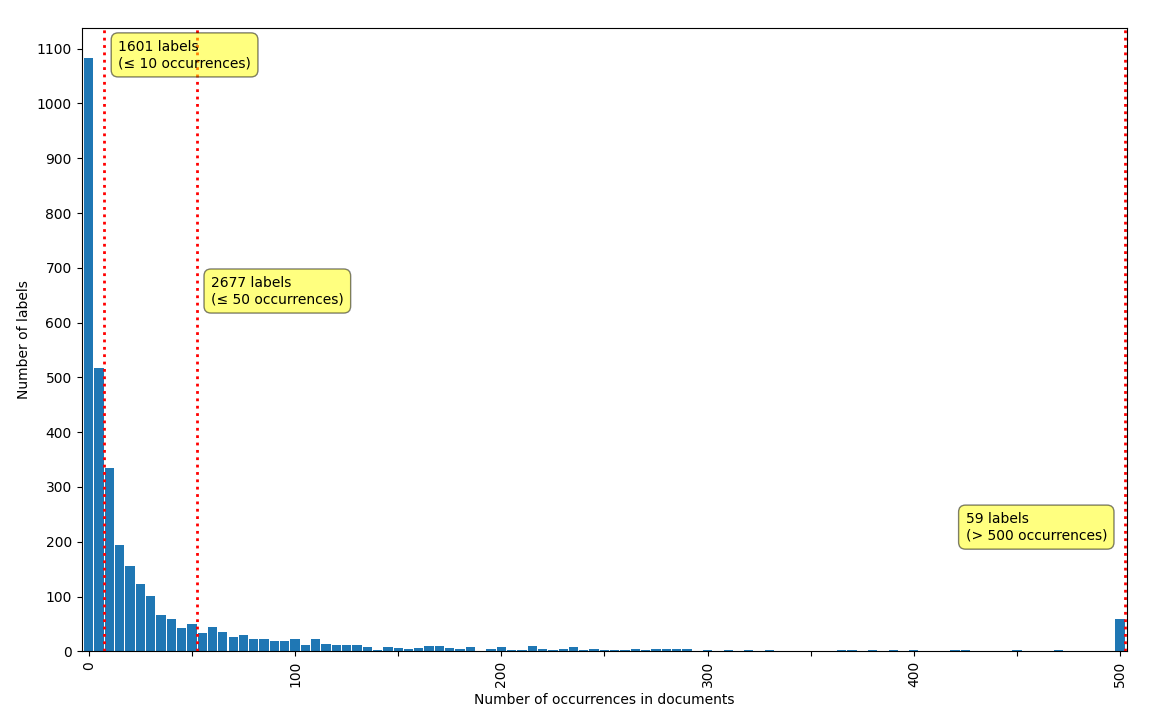
\includegraphics[width=0.8\textwidth]{figures/filtered_articles.png}
  \caption{The distribution of label occurrences in the $NewsMon_{sl+cls}$ dataset.}
  \label{fig:filtered_articles}
\end{figure}

\begin{figure}[h!]
  \centering
  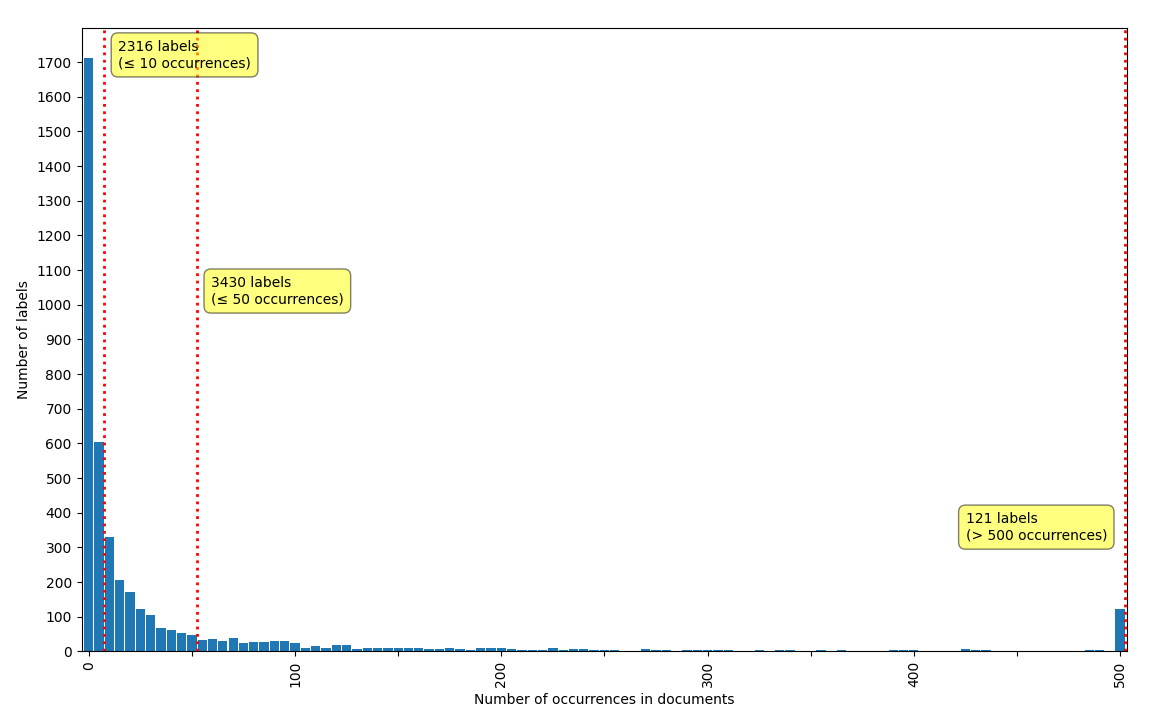
\includegraphics[width=0.8\textwidth]{figures/eurlex.png}
  \caption{The distribution of label occurrences in the $EURLEX57K$ dataset.}
  \label{fig:eurlex}
\end{figure}

The $EURLEX57K$ dataset, with 57,000 instances and 4,271 labels, has an average of 5.069 labels per instance and a label density of 0.00119, indicating a denser and more complex label distribution compared to the $NewsMon_{sl}$ datasets. 
This highlights the intricate label structure of $EURLEX57K$, while the $NewsMon_{sl+cls}$ dataset, after removing single-occurrence labels, shows a more concentrated label distribution than the unfiltered $NewsMon_{sl}$ dataset. 
A high standard deviation for cardinality in $NewsMon_{sl}$ datasets suggests that the number of labels per instance is spread out over a wider range.
Overall, the datasets show similar properties regarding the long-tail label distribution, which can be observed in Figure~\ref{fig:filtered_articles} and in Figure~\ref{fig:eurlex}.
